% SIAM Article Template
\documentclass[review,hidelinks,onefignum,onetabnum]{siamart220329}

% Information that is shared between the article and the supplement
% (title and author information, macros, packages, etc.) goes into
% ex_shared.tex. If there is no supplement, this file can be included
% directly.

% SIAM Shared Information Template
% This is information that is shared between the main document and any
% supplement. If no supplement is required, then this information can
% be included directly in the main document.


% Packages and macros go here
\usepackage{lipsum}
\usepackage{amsfonts}
\usepackage{graphicx}
\usepackage{epstopdf}
\usepackage{algorithmic}
\ifpdf
  \DeclareGraphicsExtensions{.eps,.pdf,.png,.jpg}
\else
  \DeclareGraphicsExtensions{.eps}
\fi

% Add a serial/Oxford comma by default.
\newcommand{\creflastconjunction}{, and~}

% Used for creating new theorem and remark environments
\newsiamremark{remark}{Remark}
\newsiamremark{hypothesis}{Hypothesis}
\crefname{hypothesis}{Hypothesis}{Hypotheses}
\newsiamthm{claim}{Claim}

% Sets running headers as well as PDF title and authors
\headers{A second order numerical methods for Reisz-Fractional Elliptic Equation on graded mesh }{Jianxing Han and Minghua Chen}

% Title. If the supplement option is on, then "Supplementary Material"
% is automatically inserted before the title.
\title{second-order error analysis for Fractional Laplacian via Riesz Derivatives on graded meshes\thanks{Submitted to the editors DATE.
}}

% Authors: full names plus addresses.
\author{Jianxing Han\thanks{School of Mathematics and Statistics, Lanzhou University, Lanzhou 730000, PR China
  (\email{hanjx2023@mail.lzu.edu.cn}).}
  \and Minghua Chen\thanks{School of Mathematics and Statistics, Lanzhou University, Lanzhou 730000, PR China 
  (\email{chen@mail.lzu.edu.cn}).}
}

\usepackage{amsopn}
\DeclareMathOperator{\diag}{diag}


%%% Local Variables: 
%%% mode:latex
%%% TeX-master: "ex_article"
%%% End: 


% Optional PDF information
\ifpdf
\hypersetup{
  pdftitle={An Example Article},
  pdfauthor={D. Doe, P. T. Frank, and J. E. Smith}
}
\fi

% The next statement enables references to information in the
% supplement. See the xr-hyperref package for details.

\externaldocument[][nocite]{ex_supplement}

% FundRef data to be entered by SIAM
%<funding-group specific-use="FundRef">
%<award-group>
%<funding-source>
%<named-content content-type="funder-name"> 
%</named-content> 
%<named-content content-type="funder-identifier"> 
%</named-content>
%</funding-source>
%<award-id> </award-id>
%</award-group>
%</funding-group>

\begin{document}

\maketitle

% REQUIRED
\begin{abstract}
  This is an example SIAM \LaTeX\ article. This can be used as a
  template for new articles.  Abstracts must be able to stand alone
  and so cannot contain citations to the paper's references,
  equations, etc.  An abstract must consist of a single paragraph and
  be concise. Because of online formatting, abstracts must appear as
  plain as possible. Any equations should be inline.
\end{abstract}

% REQUIRED
\begin{keywords}
  example, \LaTeX
\end{keywords}

% REQUIRED
\begin{MSCcodes}
  68Q25, 68R10, 68U05
\end{MSCcodes}

\section{Introduction}
The introduction introduces the context and summarizes the
manuscript. It is importantly to clearly state the contributions of
this piece of work.

\textcolor{blue}{
  For \(\Omega=(0,1)\), \(1<\alpha<2\), suppose \(f\in C^2(\Omega)\)
  \begin{equation} \label{eq:equation}
    \begin{cases}
      (-\Delta)^{\frac{\alpha}{2}} u(x) = f(x), & x \in \Omega                      \\
      u(x) = 0,                                 & x \in \mathbb{R} \setminus \Omega
    \end{cases}
  \end{equation}
  where
  \begin{equation} \label{def:operator}
    (-\Delta)^{\frac{\alpha}{2}} u(x) = -\frac{\partial^\alpha u}{\partial |x|^\alpha}
    = -\kappa_\alpha \frac{d^2}{dx^2} \int_\Omega \frac{u(y)}{|x-y|^{\alpha-1}} dy
  \end{equation}
  \begin{equation} \label{def:kappa}
    \kappa_\alpha = -\frac{1}{2\cos(\alpha\pi/2)\Gamma(2-\alpha)} > 0
  \end{equation}
}

% The outline is not required, but we show an example here.
The paper is organized as follows. Our main results are in
\cref{sec:main},  experimental
results are in \cref{sec:experiments}, and the conclusions follow in
\cref{sec:conclusions}.


\section{Numeric Format}
\label{sec:numformat}


\textcolor{blue}{
  \begin{equation} \label{def:xj}
    x_i = \begin{cases}
      \frac{1}{2} \left(\frac{i}{N}\right)^r   ,     & 0 \le i \le N  \\
      1 - \frac{1}{2} \left(\frac{2N-i}{N}\right)^r, & N \le i \le 2N
    \end{cases}
  \end{equation}
  where $r\ge 1$ .
  And let
  \begin{equation} \label{def:hj}
    h_j = x_{j} - x_{j-1}, \quad 1\le j \le 2N
  \end{equation}
}

\textcolor{blue}{
Let $\{\phi_j(x)\}_{j=1}^{2N-1}$ be standard hat functions, which are basis of the piecewise linear function space.
\begin{equation}
  \phi_j(x) = \begin{cases}
    \frac{1}{h_j} (x-x_{j-1}),      & x_{j-1} \le x \le x_{j} \\
    \frac{1}{h_{j+1}} (x_{j+1}-x) , & x_{j} \le x \le x_{j+1} \\
    0,                              & \text{otherwise}
  \end{cases}
\end{equation}
And then, we can approximate $u(x)$ with
\begin{equation}
  u_h(x) := \sum_{j=1}^{2N-1} u(x_j) \phi_j(x)
\end{equation}
}

\textcolor{blue}{
For convience, we denote
\begin{equation} \label{def:Ih}
  I_h(x) := \int_{\Omega} |x-y|^{1-\alpha} u_h(y) dy
\end{equation}
And now, we can approximate the operator \eqref{def:operator} at $x_i$ with
\begin{equation} \label{def:Dhalpha}
  D_h^{\alpha} u_h(x_i) := -\kappa_\alpha \frac{2}{h_{i} + h_{i+1}} 
  \left( \frac{1}{h_{i}} I_h(x_{i-1}) - \left( \frac{1}{h_{i}} + \frac{1}{h_{i+1}} \right) I_h(x_{i}) + \frac{1}{h_{i+1}} I_h(x_{i+1}) \right)
\end{equation}
Finally, we approximate the equation \eqref{eq:equation} with
\begin{equation} \label{def:discrete_equation}
  D_h^{\alpha} u_h(x_i) = f(x_i), \quad 1\le i \le 2N-1
\end{equation}
}


\textcolor{blue}{
  The discrete equation \eqref{def:discrete_equation} can be written in matrix form
  \begin{equation}
    AU = F
  \end{equation}
  where $U$ is unknown, $F=(f(x_1), \cdots, f(x_{2N-1}))$.
  The matrix $A$ is constructed as follows:
  Since
  \begin{equation}
    \begin{aligned} \label{eq:Ih}
      I_h(x_i) &= \int_{\Omega} |x_i-y|^{1-\alpha} u_h(y) dy 
      = \sum_{j=1}^{2N-1} \int_{\Omega} |x_i-y|^{1-\alpha} u(x_j) \phi_j(y) dy  \\
      &= \sum_{j=1}^{2N-1} u(x_j)  \int_{x_{j-1}}^{x_{j+1}} |x_i-y|^{1-\alpha} \phi_j(y) dy \\
      &= \sum_{j=1}^{2N-1} \frac{u(x_j)}{(2-\alpha)(3-\alpha)} 
      \left( \frac{|x_{i}-x_{j-1}|^{3-\alpha}}{h_{j}} -\frac{h_{j} + h_{j+1}}{h_{j}h_{j+1}}|x_i-x_{j}|^{3-\alpha} +  \frac{|x_{i}-x_{j+1}|^{3-\alpha}}{h_{j+1}} \right) \\
      & =: \sum_{j=1}^{2N-1} \tilde{a}_{ij} \; u(x_j), \quad 0 \le i \le 2N
    \end{aligned}
  \end{equation}
  Then, substitute in \eqref{def:Dhalpha}, we have
  \begin{equation}
    D_h^{\alpha} u_h(x_i) = \sum_{j=1}^{2N-1} a_{ij} \; u(x_j)
  \end{equation}
  where
  \begin{equation} \label{mat:aij}
    a_{ij} = -\kappa_\alpha \frac{2}{h_{i} + h_{i+1}} 
    \left( \frac{1}{h_{i}} \tilde{a}_{i-1,j} - \left( \frac{1}{h_{i}} + \frac{1}{h_{i+1}} \right) \tilde{a}_{i,j} +  \frac{1}{h_{i+1}} \tilde{a}_{i+1, j} \right)
  \end{equation}
}


\section{Main results}
\label{sec:main}


Here we state our main results; the proof is
deferred to \cref{sec:proof}.

\textcolor{blue}{
\begin{theorem}[truncation error] \label{thm:truncation-error}
  If $f \in C^2(\Omega)$ and $\alpha\in(1,2)$, then there exists a constant
  $C=C(\alpha, r, \|f\|_{C^2(\Omega)})$, such that
  the truncation error of the discrete format
\end{theorem}
}

\begin{theorem}[Mean Value Theorem]\label{thm:mvt}
  Suppose $f$ is a function that is continuous on the closed interval
  $[a,b]$.  and differentiable on the open interval $(a,b)$.
  Then there exists a number $c$ such that $a < c < b$ and
  \begin{displaymath}
    f'(c) = \frac{f(b)-f(a)}{b-a}.
  \end{displaymath}
  In other words,
  \begin{displaymath}
    f(b)-f(a) = f'(c)(b-a).
  \end{displaymath}
\end{theorem}



\begin{corollary}\label{cor:a}
  Let $f(x)$ be continuous and differentiable everywhere. If $f(x)$
  has at least two roots, then $f'(x)$ must have at least one root.
\end{corollary}
\begin{proof}
  Let $a$ and $b$ be two distinct roots of $f$.
  By \cref{thm:mvt}, there exists a number $c$ such that
  \begin{displaymath}
    f'(c) = \frac{f(b)-f(a)}{b-a} = \frac{0-0}{b-a} = 0.
  \end{displaymath}
\end{proof}

Note that it may require two \LaTeX\ compilations for the proof marks
to show.

Display matrices can be rendered using environments from \texttt{amsmath}:
\begin{equation}\label{eq:matrices}
  S=\begin{bmatrix}1&0\\0&0\end{bmatrix}
  \quad\text{and}\quad
  C=\begin{pmatrix}1&1&0\\1&1&0\\0&0&0\end{pmatrix}.
\end{equation}
Equation \cref{eq:matrices} shows some example matrices.

We calculate the Fr\'{e}chet derivative of $F$ as follows:
\begin{subequations}
  \begin{align}
    F'(U,V)(H,K)
     & = \langle R(U,V),H\Sigma V^{T} + U\Sigma K^{T} -
    P(H\Sigma V^{T} + U\Sigma K^{T})\rangle \label{eq:aa}    \\
     & = \langle R(U,V),H\Sigma V^{T} + U\Sigma K^{T}\rangle
    \nonumber                                                \\
     & = \langle R(U,V)V\Sigma^{T},H\rangle +
    \langle \Sigma^{T}U^{T}R(U,V),K^{T}\rangle. \label{eq:bb}
  \end{align}
\end{subequations}
\Cref{eq:aa} is the first line, and \cref{eq:bb} is the last line.

\section{Algorithm}
\label{sec:alg}

\lipsum[40]

Our analysis leads to the algorithm in \cref{alg:buildtree}.

\begin{algorithm}
  \caption{Build tree}
  \label{alg:buildtree}
  \begin{algorithmic}
    \STATE{Define $P:=T:=\{ \{1\},\ldots,\{d\}$\}}
    \WHILE{$\#P > 1$}
    \STATE{Choose $C^\prime\in\mathcal{C}_p(P)$ with $C^\prime := \operatorname{argmin}_{C\in\mathcal{C}_p(P)} \varrho(C)$}
    \STATE{Find an optimal partition tree $T_{C^\prime}$ }
    \STATE{Update $P := (P{\setminus} C^\prime) \cup \{ \bigcup_{t\in C^\prime} t \}$}
    \STATE{Update $T := T \cup \{ \bigcup_{t\in\tau} t : \tau\in T_{C^\prime}{\setminus} \mathcal{L}(T_{C^\prime})\}$}
    \ENDWHILE
    \RETURN $T$
  \end{algorithmic}
\end{algorithm}

\lipsum[41]

\section{Experimental results}
\label{sec:experiments}

\lipsum[50]

\Cref{fig:testfig} shows some example results. Additional results are
available in the supplement in \cref{tab:foo}.

\begin{figure}[htbp]
  \centering
  \label{fig:a}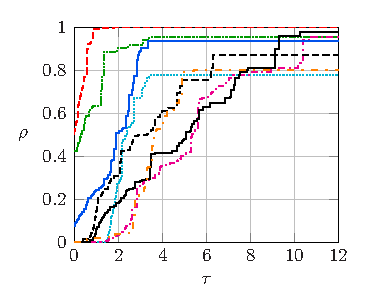
\includegraphics{lexample_fig1}
  \caption{Example figure using external image files.}
  \label{fig:testfig}
\end{figure}

\Cref{tab:foo} shows additional
supporting evidence.

\begin{table}[htbp]
  \footnotesize
  \caption{Example table.}\label{tab:foo}
  \begin{center}
    \begin{tabular}{|c|c|c|} \hline
      Species & \bf Mean & \bf Std.~Dev. \\ \hline
      1       & 3.4      & 1.2           \\
      2       & 5.4      & 0.6           \\
      3       & 7.4      & 2.4           \\
      4       & 9.4      & 1.8           \\ \hline
    \end{tabular}
  \end{center}
\end{table}

\lipsum[51]

\section{Discussion of \texorpdfstring{{\boldmath$Z=X \cup Y$}}{Z = X union Y}}

\lipsum[76]

\section{Conclusions}
\label{sec:conclusions}

Some conclusions here.


\appendix
\section{An example appendix}
\lipsum[71]

\begin{lemma}
  Test Lemma.
\end{lemma}

\section*{Acknowledgments}
We would like to acknowledge the assistance of volunteers in putting
together this example manuscript and supplement.

\bibliographystyle{siamplain}
\bibliography{references}
\end{document}
